\begingroup
\small
\begin{frame}
\frametitle{Методы восстановления}
\begin{tabular}{p{0.15\textwidth} | p{0.4\textwidth} | p{0.4\textwidth}}
\hspace{-1cm} семейство & Интегральные & Алгебраические \\ \hline
\hspace{-1cm} подход & Аналитическая формула для обращения $R^{-1}[p(\varphi, \xi)](x,y)$ & Оптимизационная задача $\min_{f} \Norm{R[f] - p}$\\ \hline
\hspace{-1cm} представители & FBP & ART, SART, SIRT \\ \hline
\hspace{-1cm} сложность & $O(N^2 \log N)$ & $O(N^3)$ \\ \hline
\hspace{-1cm} особенности & универсальность & возможность учета \hspace{1cm} модели объекта или измерительной схемы \\
                          & требует полного набора проекционных углов, & \\ 
                          & их равномерного распределения & \\
                          & чувствительны к шумам & \\
\end{tabular}
\\
\vspace{0.5cm}

$N$ --- число ячеек детектора
\end{frame}
\endgroup


%\section{Вычислительно эффективный алгебраический метод восстановления FHT-SIRT}

\begin{frame}
\frametitle{Алгебраический метод}
\framesubtitle{Основные положения}
\begin{itemize}
  \item непрерывные функции $\rightarrow$ дискретные изображения:

    {
    \centering
    $f(x,y) \rightarrow f_i,\ p(\varphi, s) \rightarrow p_j$
    \par
    }
  \vspace{0.5cm}
  \item преобразование Радона $\rightarrow$ преобразование Хафа:
  
    {
    \centering
    $R[f](\varphi, s) \rightarrow (\mathrm W f)_j$ 
    \par
    }
  \vspace{0.5cm}

    $\mathrm W$ - матрица проекции, указывает вклад пикселя $i$ в лучевую сумму вдоль луча $j$.
    Разреженная матрица размера $N_\varphi * N^3$, в которой только порядка $O(N_\varphi * N^2)$ ненулевых элементов
    \vspace{0.5cm}
  \item решение разреженной СЛАУ большой размерности итерационным методом

    {
    \centering
    $p = \mathrm W f$
    \par
    }

\end{itemize}
\end{frame}

\begin{frame}
\frametitle{Матрица проекции W}
\begin{tabular}{c c c}
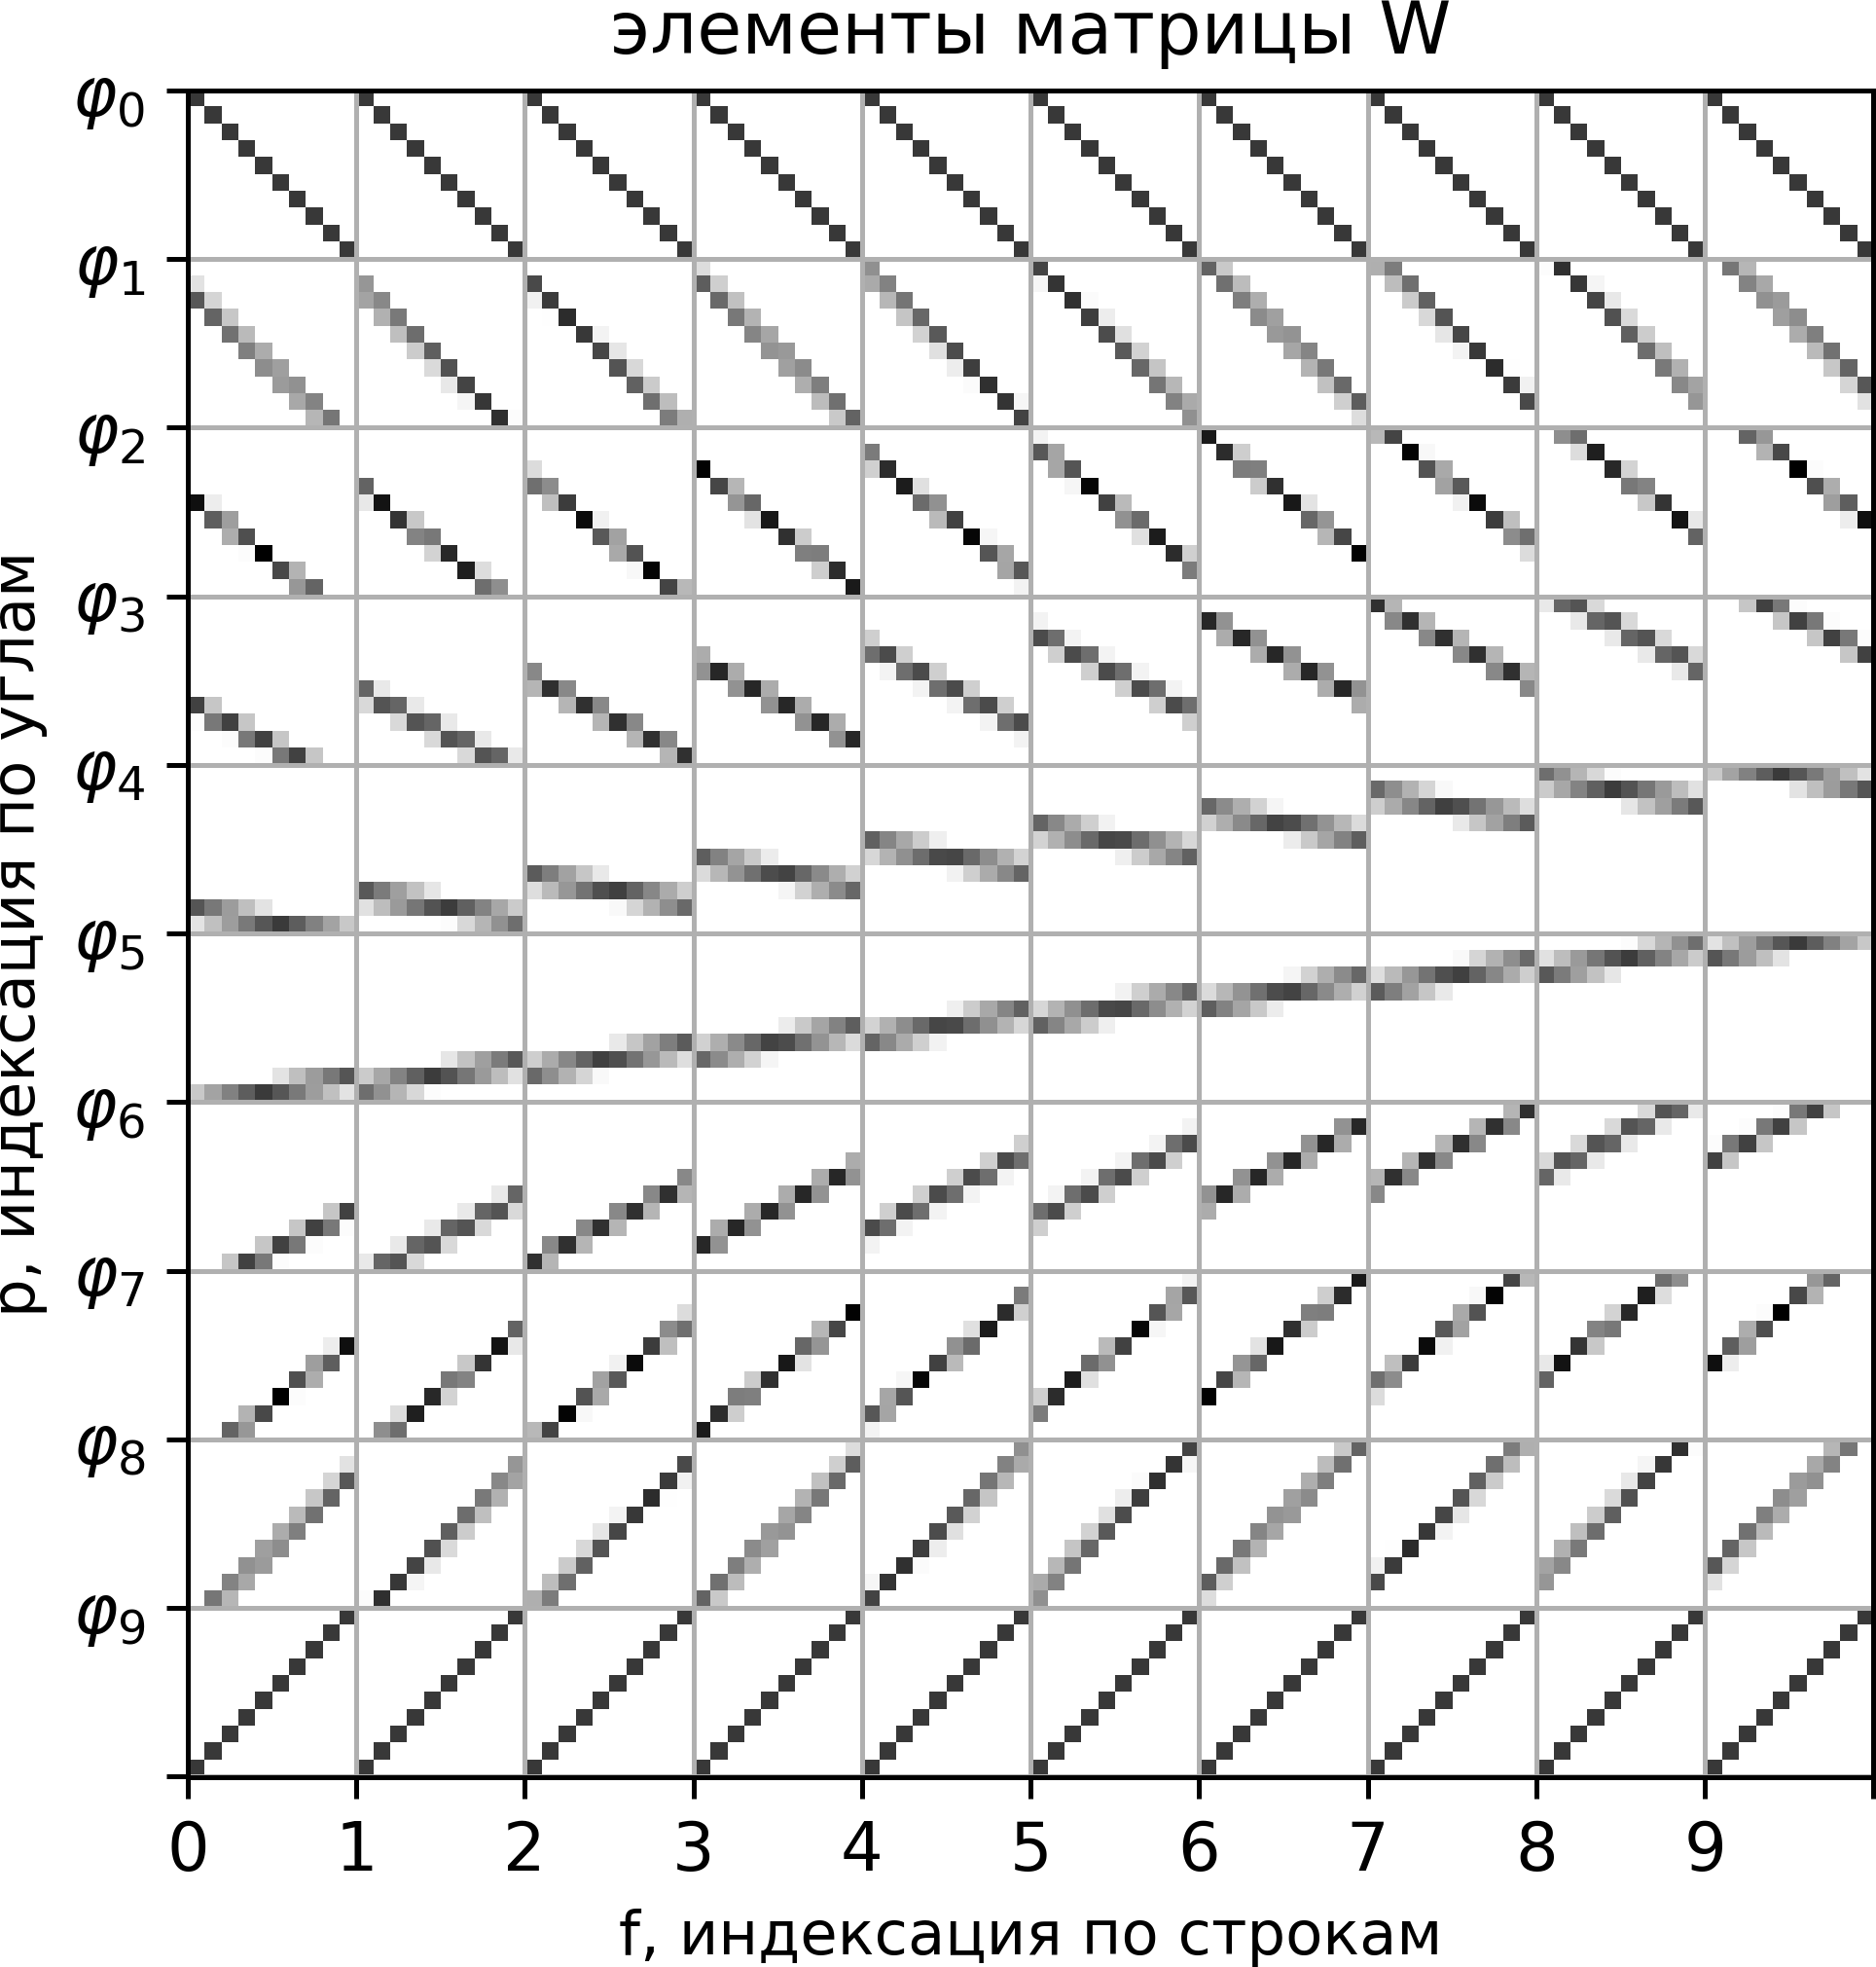
\includegraphics[width=0.4\textwidth]{w_matrices/W_10_10_plot.png} &
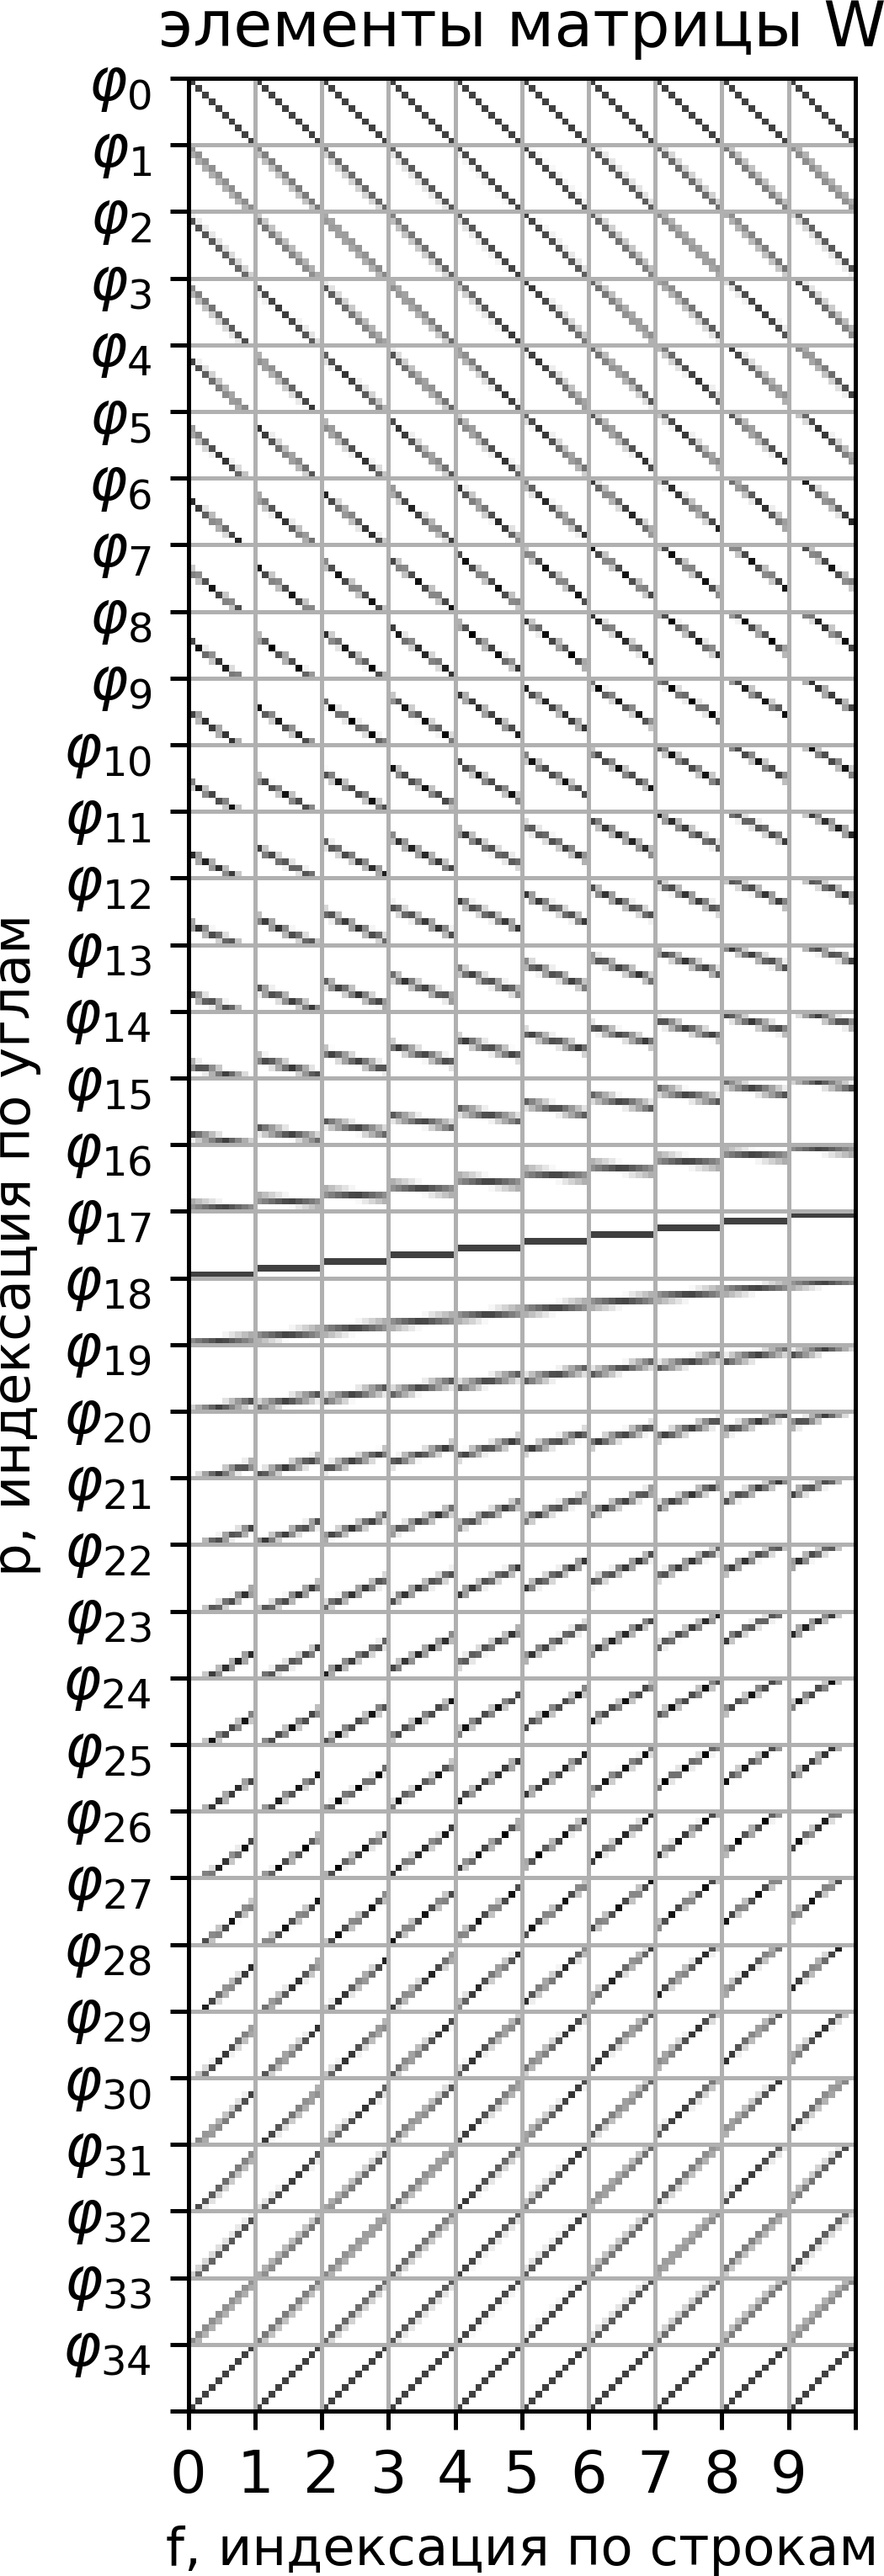
\includegraphics[height=0.8\textheight]{w_matrices/W_10_35_plot.png} &
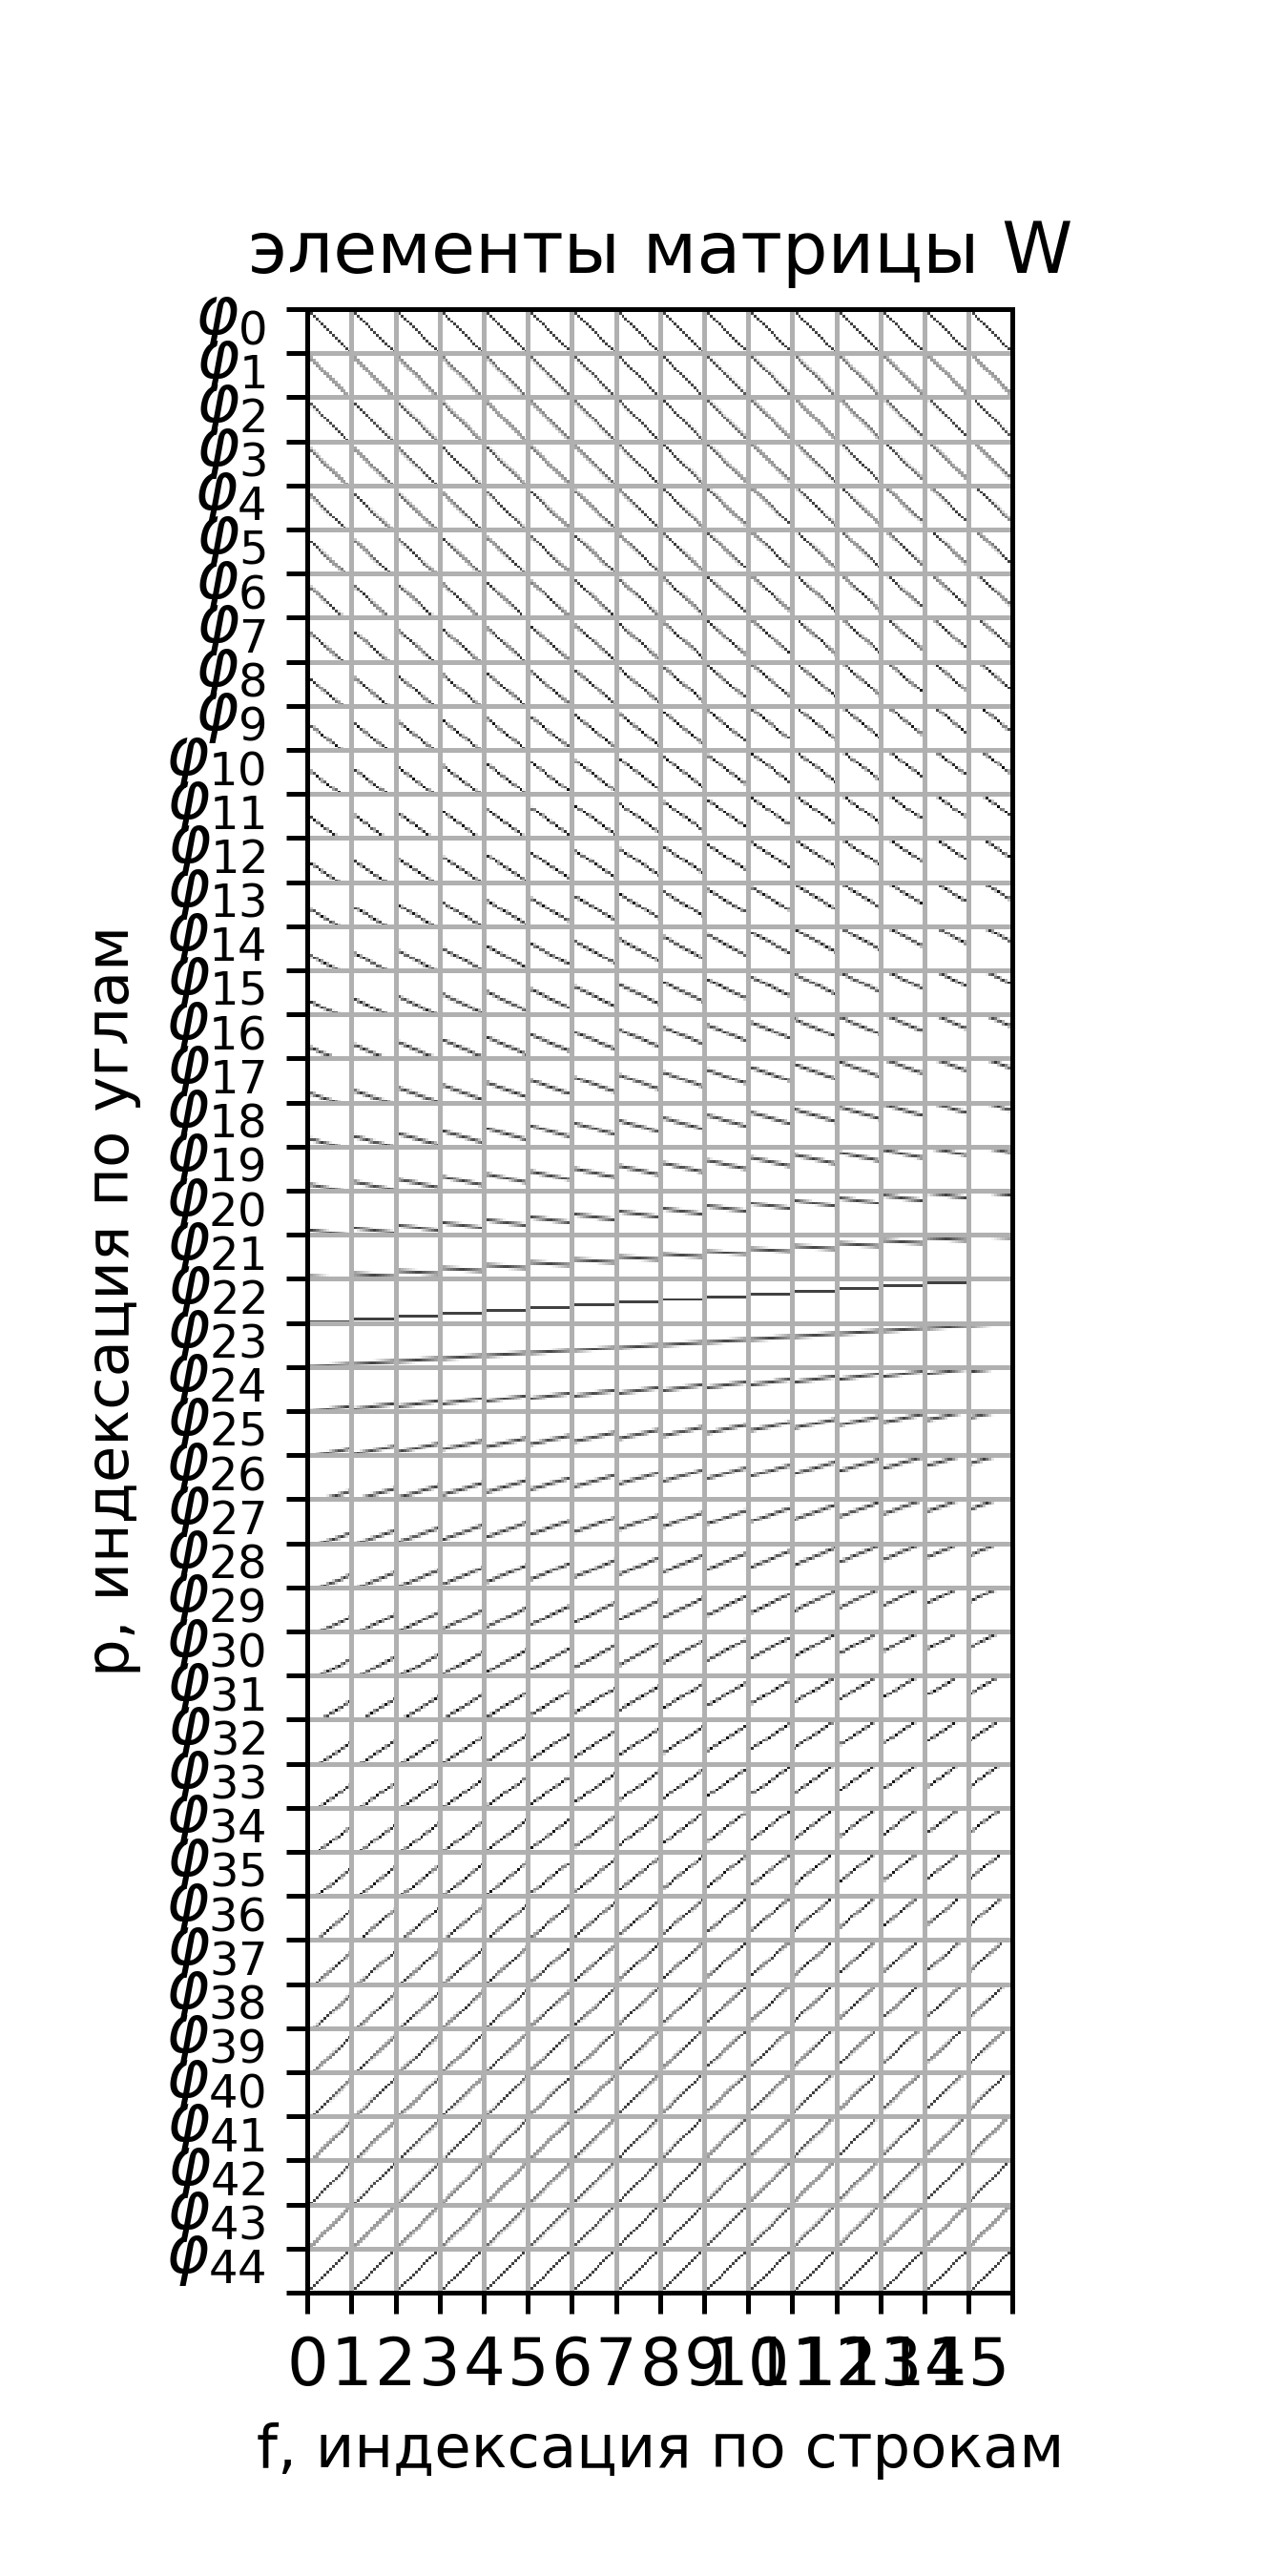
\includegraphics[height=0.8\textheight]{w_matrices/W_16_45_plot.png} \\
\small{$N = 10$, $N_\varphi = 10$} &
\small{$N = 10$, $N_\varphi = 35$} & 
\small{$N = 16$, $N_\varphi = 45$}
\end{tabular}
\end{frame}

\begin{frame}
\frametitle{Алгебраический метод}
\framesubtitle{Решение СЛАУ}
\centering
$\Norm{p - \mathrm W f} \rightarrow \min\limits_f$

Оптимизационная задача решается итерационным методом, шаг итерации имеет вид
\vspace{0.5cm}

\begingroup
\footnotesize

\hspace*{-0.5cm}
\begin{tabular}{c|c|c}
ART & SART & SIRT \\ \hline
для каждого луча & для каждого угла & для всех лучей\\
$j = 1 \dots N * N_\varphi$ & $\varphi_k$ & \\
$\hat{f} = f - \gamma \mathrm W^{\mathrm T}_j(\mathrm W f - p)$ &
$\hat{f} = f - \gamma \mathrm {W^{\varphi_k}}^{\mathrm T}(\mathrm W f - p)$ &
$\hat{f} = f - \gamma \mathrm W^{\mathrm T}(\mathrm W f - p)$ \\
\end{tabular}

\vspace{0.5cm}
\raggedright
\endgroup

$\mathrm W_j$ --- столбец матрицы для луча $j$,\\
$\mathrm W^\varphi$ ---  матрица проекции на угол $\varphi$, $\mathrm W = \sum_\varphi {\mathrm W^\varphi}$


\end{frame}